\documentclass[11pt]{beamer}
\usetheme{Warsaw}
\mode<presentation>{}
\usepackage[utf8]{inputenc}
\usepackage[english]{babel}
\usepackage{amsmath}
\usepackage{amsfonts}
\usepackage{amssymb}
\usepackage{graphicx}
\usepackage{listings}
\usepackage{todonotes}
\usepackage{lmodern}
\usepackage{infer}

\author{Enrico Steffinlongo}
\title{Privilege separation in browser architectures}
\institute[Universities Here and There] % (optional)
{
  Università Ca' Foscari - Computer science
}
%\date{}


%\setbeamercovered{transparent} 
\setbeamertemplate{navigation symbols}{} 
%\logo{} 
%\institute{} 
%\date{} 
%\subject{} 

\defbeamertemplate*{footline}{shadow theme}
{%
  \leavevmode%
  \hbox{\begin{beamercolorbox}[wd=.5\paperwidth,ht=2.5ex,dp=1.125ex,leftskip=.3cm plus1fil,rightskip=.3cm]{author in head/foot}%
    \hfill\insertshortauthor
  \end{beamercolorbox}%
  \begin{beamercolorbox}[wd=.5\paperwidth,ht=2.5ex,dp=1.125ex,leftskip=.3cm,rightskip=.3cm plus1fil]{title in head/foot}%
    \usebeamerfont{title in head/foot}\insertshorttitle\hfill\insertframenumber\,/\,\inserttotalframenumber%
  \end{beamercolorbox}}%
  \vskip0pt%
}

% basics
\newcommand{\names}{\mathcal{N}}
\newcommand{\vars}{\mathcal{V}}
\newcommand{\perms}{\mathcal{P}}
\newcommand{\refs}{\mathcal{R}}
\newcommand{\caller}{\mathbf{caller}}

\renewcommand{\vec}[1]{\overrightarrow{#1}}
\newcommand{\subst}[2]{[#1/#2]}
\newcommand{\overwrite}[2]{[#1 \mapsto #2]}
\newcommand{\xra}[1]{\xrightarrow{#1}}
\newcommand{\xRa}[1]{\xRightarrow{#1}}
\newcommand{\hra}{\hookrightarrow}
\newcommand{\fv}{\mathit{fv}}
\newcommand{\fn}{\mathit{fn}}
\newcommand{\fnfv}{\mathit{fnfv}}
\newcommand{\map}[3]{#1 \stackrel{#2}{\mapsto} #3}
\newcommand{\dom}{\mathit{dom}}
\newcommand{\defined}[1]{#1\!\downarrow\ }

\newcommand{\powerset}[1]{2^{#1}}
\newcommand{\jm}{\mathcal{J}}
\newcommand{\fvbv}{\mathit{vars}}

\newenvironment{mcases}[0]{\begin{list}{{\em Case}}{\leftmargin 5pt}}{\end{list}}

% permission
\newcommand{\join}{\sqcup}
\newcommand{\meet}{\sqcap}
\newcommand{\compl}[1]{#1^*}

% values
\newcommand{\lam}[2]{\lambda #1.#2}
\newcommand{\rec}[1]{\{#1\}}
\newcommand{\unit}{\mathbf{unit}}
\newcommand{\true}{\mathbf{true}}
\newcommand{\false}{\mathbf{false}}
\newcommand{\str}[1]{``\mathit{#1}''}
\newcommand{\undef}{\mathbf{undefined}}

% expressions
\newcommand{\letexpr}[3]{\mathbf{let}\ #1 = #2\ \mathbf{in}\ #3}
\newcommand{\appl}[2]{#1\, #2}
\newcommand{\op}{\mathit{op}}
\newcommand{\cond}[3]{\mathbf{if}\ (#1)\ \{\ #2\ \}\ \mathbf{else}\ \{\ #3\ \}}
\newcommand{\while}[2]{\mathbf{while}\ (#1)\ \{\ #2\ \}}
\newcommand{\lookup}[2]{#1[#2]}
\newcommand{\store}[3]{#1[#2] = #3}
\newcommand{\delete}[2]{\mathbf{delete}\ #1[#2]}
\newcommand{\err}{\mathbf{err}}
\newcommand{\newref}[2]{\mathbf{ref}_{#1}\ #2}
\newcommand{\deref}[1]{\mathbf{deref}\ #1}
\newcommand{\setref}[2]{#1 = #2}
\newcommand{\send}[3]{\overline{#1} \langle #2 \triangleright #3 \rangle}
\newcommand{\checkperms}[2]{\mathbf{check}(#1,#2)}
\newcommand{\acquire}[1]{\mathbf{acquire}(#1)}
\newcommand{\release}[1]{\mathbf{release}(#1)}
\newcommand{\register}[3]{\mathbf{register}(#1,#2,#3)}
\newcommand{\exercise}[1]{\mathbf{exercise}(#1)}
\newcommand{\self}{\mathbf{self}}

\newcommand{\match}[2]{\mathbf{match}\ #1\ \mathbf{with}\ \{#2\}}
\newcommand{\checkp}[3]{\mathbf{check}(#1)\ \mathbf{then}\ #2\ \mathbf{else}\ #3}

% components, systems and states
\newcommand{\handler}[5]{#1(#2 \triangleleft #3:#5).#4}
\newcommand{\inst}[3]{#1\{\!|#2|\!\}_{#3}}
\newcommand{\para}[2]{#1 \parallel #2}
\newcommand{\sys}[3]{#1;#2;#3}

\newcommand{\ctx}[2]{#1\langle #2\rangle}
\newcommand{\labcall}[4]{\langle #1:#2,#3:#4 \rangle}
\newcommand{\labex}[3]{#1:#2 \gg #3}

% misc
\newcommand{\lambdaJS}{\lambda_{\mathsf{JS}}}
\newcommand{\irule}[1]{({\sc #1})}

% flow logic
\newcommand{\labs}{{\mathcal L}}
\newcommand{\absenv}{\hat{\Gamma}}
\newcommand{\absflow}{\hat{\phi}}
\newcommand{\absnet}{\hat{\Phi}}
\newcommand{\absvalues}{\hat{V}}
\newcommand{\absmem}{\hat{\mu}}
\newcommand{\abscache}{\hat{\Phi}}
\newcommand{\absassert}{\hat{L}}
\newcommand{\forms}{\Phi}
\newcommand{\terms}{\mathcal{T}}

\newcommand{\absop}{\widehat{\op}}
\newcommand{\abseq}{\widehat{eq}}
\newcommand{\absget}{\widehat{get}}
\newcommand{\absset}{\widehat{set}}
\newcommand{\absdel}{\widehat{del}}

\newcommand{\dontcare}{\diamond}
\newcommand{\abscaller}{\widehat{\caller}}
\newcommand{\msg}{\mathbb{M}}
\newcommand{\abself}{\widehat{\self}}
\newcommand{\absform}[1]{\langle #1 \rangle}
\newcommand{\hasperm}[2]{#1\ \mathsf{has}\ #2}
\newcommand{\ltrue}{\mathsf{true}}
\newcommand{\lacquire}[3]{#1 \uparrow #2,#3}
\newcommand{\lrelease}[3]{#1 \downarrow #2,#3}
\newcommand{\abstrue}{\true}
\newcommand{\absfalse}{\false}
\newcommand{\absunit}{\unit}
\newcommand{\absundef}{\undef}
\newcommand{\absrec}[1]{\langle\!| #1 |\!\rangle}
\newcommand{\abslam}[2]{\lambda #1^{#2}}
\newcommand{\absfuns}{\Lambda}

\newcommand{\absC}{{\cal C}}

% debundling
\newcommand{\avail}[1]{\mathit{Avail}_{#1}}
\newcommand{\req}[1]{\mathit{Req}_{#1}}
\newcommand{\psubst}[3]{[#1/#2]@#3}
\newcommand{\unbundle}[3]{#1 \rhd_{#2}\, #3}
\newcommand{\absE}{{\cal E}}
\newcommand{\rewrite}[1]{\succ #1}

% escalation
\newcommand{\abstack}{\hat{\Upsilon}}
\newcommand{\escalate}[1]{\,\gg #1}
\newcommand{\despite}[1]{\ \mathbf{despite}\ #1}
\newcommand{\permsleak}[1]{\mathit{Leak}_{#1}}

%other mine
\newcommand{\vat}[0]{\hat{v}}
\newcommand{\ljs}{$\lambda_{JS}$}

\begin{document}

\begin{frame}
\titlepage
\end{frame}

%\begin{frame}
%\listoftodos
%\end{frame}

\begin{frame}
\tableofcontents
\end{frame}

%\section{Intro}
%%\subsection{Browser extensions}
\begin{frame}{Browser Extensions}
Web browsers extensions are phenomenally popular.
\begin{itemize}
\item roughly 33\% of Firefox users have at least one add-on
\end{itemize}
Extension customize the user experience
\begin{itemize}
\item Customize the user interface
\item Adds lots of functionality to the browser (e.g., save and restore tabs)
\item Protect users from certain contents of the web pages 
\end{itemize}
\end{frame}

\begin{frame}{Browser Extensions}
Extension need to interact with
\begin{itemize}
\item Web pages DOM
\item Browser internal structure (tabs collections, \dots)
\item Browser API (browser storage, cookie jar, \dots)
\end{itemize}
Potential security problem!
\begin{itemize}
\item Browser API $\Rightarrow$ security critical operations\\
\item Web interaction $\Rightarrow$ Untrusted and potentially malicious\\
\end{itemize}
\end{frame}

%\subsection{Chrome Extension}

\begin{frame}{Chrome extensions architecture}
\begin{columns}[T]
\begin{column}{.48\textwidth}
Chrome extension architecture force developers to three practices
\begin{enumerate}
\item Privilege separation
\item Least privilege
\item Strong isolation
\end{enumerate}
\end{column}%
\begin{column}{.48\textwidth}
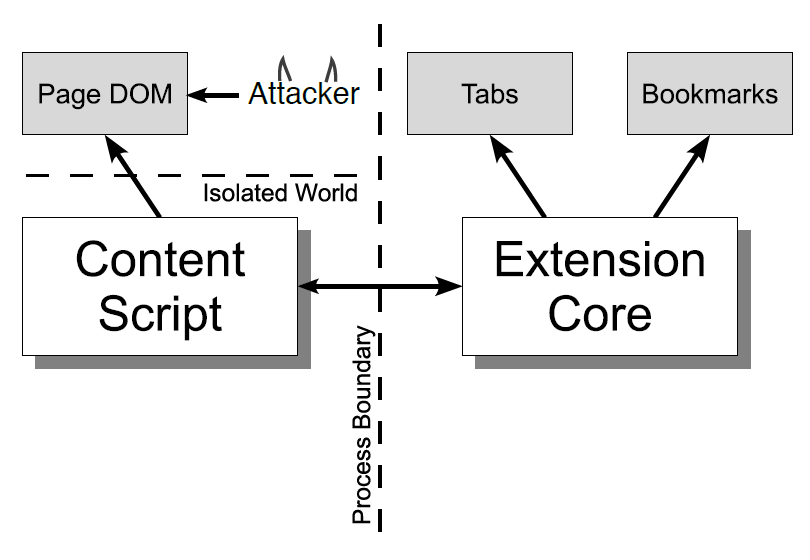
\includegraphics[scale=0.25]{Images/StrongIsolation.png}
\end{column}%
\end{columns}
\end{frame}

\begin{frame}{Privilege separation}
\begin{itemize}
\item Content scripts
\begin{itemize}
\item Injected to each page (multiple instances)
\item Access the DOM of the page
\item Cannot use privileges other than the one used to send messages to the Extension Core
\end{itemize}
\item Extension Core
\begin{itemize}
\item Single instance for each browser session
\item No access to DOM of pages
\item Can use privileges defined statically in the manifest
\end{itemize}
\end{itemize}
\end{frame}

\begin{frame}{Least privilege}
An extension has a limited set of permission defined statically in the manifest
\begin{itemize}
\item An extension cannot use more than required permissions
\item User have to agree with the required permission at install time
\item Attacker cannot use more than such set of privileges
\end{itemize}
\end{frame}

\begin{frame}{Strong isolation}
All components of the extension have different address spaces except content scripts that can read and modify the DOM of the page on which are injected. So an infected component could not
\begin{itemize}
\item alter content of variables of other components
\item invoke or alter functions defined in other components.
\end{itemize}

Communication between Extension Core and Content Scripts is only via message passing:
\begin{itemize}
\item Messages exchanged can only be string (Objects are marshaled using a JSON serializer)
\item Functions cannot be sent.
\end{itemize}
\end{frame}

%\begin{frame}{Isolated worlds}
%\begin{columns}[T]
%\begin{column}{.62\textwidth}
%\begin{itemize}
%\item Content script and web pages has different memory spaces
%\item Only standard DOM fields are shared
%\end{itemize}
%A potentially malign web page cannot:
%\begin{itemize}
%\item alter the content of variables of the content script
%\item invoke or share function with the content script
%\end{itemize}
%\end{column}%
%\begin{column}{.33\textwidth}
%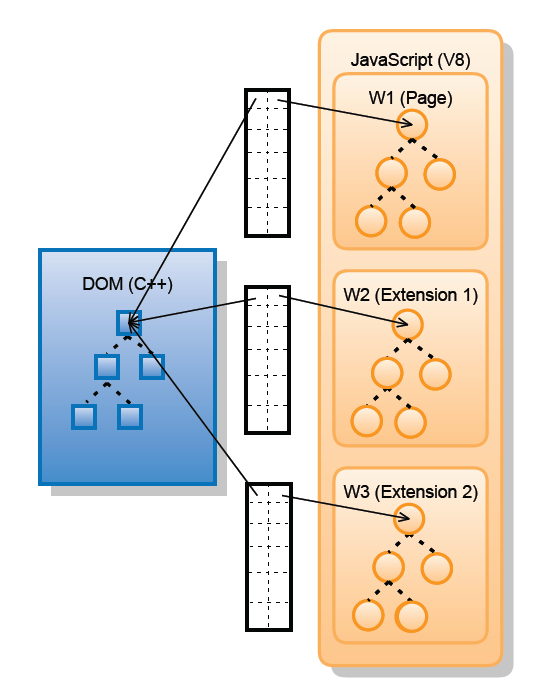
\includegraphics[scale=0.28]{Images/IsolatedWorlds.png}
%\end{column}%
%\end{columns}
%\end{frame}

\begin{frame}{Message passing}
\todo[inline]{to be fixed MPI}
Chrome extension message passing API
\end{frame}

\begin{frame}[fragile]{Example}
\todo[inline]{to be fixed Example}
\begin{columns}[T]
\begin{column}{.48\textwidth}

\end{column}
\begin{column}{.48\textwidth}
\begin{tiny}
\begin{lstlisting}
chrome.runtime.onMessage.addListener(
  function (msg, sender, sendResp) {
    if (msg.tag == "req") {
      var u = DB.getUser(msg.site);
      var p = DB.getPwd(msg.site);
      sendResp({"user": u, "pwd": p});
    }
    else if (msg.tag == "sync") {
      var db = DB.serialize();
      xmlhttp.open("GET", msg.site + db);
      xmlhttp.send();
    }
    else
      console.log ("Invalid message");
});
\end{lstlisting}
\end{tiny}
\end{column}
\end{columns}
\end{frame}


\begin{frame}{LambdaJS (Brown university\cite{LambdaJS})}
\begin{columns}[T]
\begin{column}{.48\textwidth}
JavaScript:
\begin{itemize}
\item Complex language
\item Lots of constructs
\item unconventional semantics.
\end{itemize}
Very complex to analyze!!
\end{column}
\begin{column}{.50\textwidth}
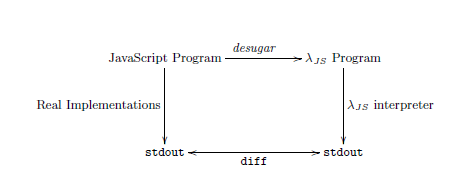
\includegraphics[scale=0.42]{Images/LambdaJS.PNG}
\end{column}
\end{columns}\vspace{0.5cm}

\ljs\cite{LambdaJS} is a core calculus made by Brown university designed specifically to ``desugar'' JavaScript
\begin{itemize}
\item Few constructs
\item Standard $\lambda$-style semantics
\item Not a sound approximation of JavaScript
\item Tests on ``desugared'' files shows that its the semantic coincide with JavaScript
\end{itemize}
Easy to analyze
\end{frame}

\begin{frame}{The calculus}
\ljs++ is an extension of \ljs\ with constructs specific for communications of components in privilege-separated architectures. Its components are:

\begin{itemize}
\item Constants: $c ::= \mathit{num} ~|~ \mathit{str} ~|~ \mathit{bool} ~|~ \unit ~|~ \undef$
\item Values: $v ::= n ~|~ x ~|~ c ~|~ r_{\ell} ~|~ \lam{x}{e} ~|~ \rec{\vec{str_i:v_i}}$
\item Expressions: classical lambda calculus construct, operations on objects and on references, $e ::= \dots |~ \newref{\ell}{e} ~|~ \send{e}{e}{\rho} ~|~ \exercise{\rho}.$
\item Memories: $\mu ::= \emptyset ~|~ \mu, \map{r_{\ell}}{\rho}{v}$
\item Handlers: $h ::= \emptyset ~|~ h,\handler{a}{x}{\rho}{e}{\rho'}$
\item Instances: $i ::= \emptyset ~|~ i,\inst{a}{e}{\rho}$
\item System: $s = \sys{\mu}{h}{i}$
\end{itemize}
\end{frame}

\begin{frame}{Judgments}
For the analysis we used the Flow logic \cite{FlowLogic} approach.
\begin{itemize}
\item All values are abstracted assuming a pre-order relation $\sqsubseteq$. $v \rightsquigarrow \hat{v}$
\item Abstract environment $\absC=\abstack ; \absnet ; \absenv ; \absmem$ is a four-tuple made of the following components:
$$
\begin{array}{llcl}
\mathit{Abstract\ variable\ environment} & \absenv & : & \vars \cup \absfuns \rightarrow \absvalues \\
\mathit{Abstract\ memory} & \absmem & : & \labs \times \perms \rightarrow \absvalues \\
\mathit{Abstract\ stack} & \abstack & : & \names \times \perms \rightarrow \perms \times \perms \\
\mathit{Abstract\ network} & \absnet & : & \names \times \perms \rightarrow \absvalues.
\end{array}
$$
\end{itemize}
We do not fix any specific representation of the domains.
\end{frame}

\begin{frame}
Each judgment of our specification has the form: 
\begin{itemize}
\item $\absC \Vdash_\rho v \rightsquigarrow \hat{v}$
\item $\absC  \Vdash_\rho e: \hat{v} \escalate{\rho'}$
\item $\absC \Vdash \mu \despite{\rho}$, $\absC \Vdash h \despite{\rho}$, 
$\absC \Vdash i \despite{\rho}$, $\absC \Vdash s \despite{\rho}$.
\end{itemize}

Example:

$$\inferrule*[width=10em,lab=(PE-Cond)]
{\absC \Vdash_{\rho_s} e_0: \hat{v}_0 \escalate{\rho_0} \sqsubseteq \rho \\
\abstrue \in \hat{v}_0 \Rightarrow \absC \Vdash_{\rho_s} e_1: \hat{v}_1 \sqsubseteq \hat{v} \escalate{\rho_1} \sqsubseteq \rho \\
\absfalse \in \hat{v}_0 \Rightarrow \absC \Vdash_{\rho_s} e_2: \hat{v}_2 \sqsubseteq \hat{v} \escalate{\rho_2} \sqsubseteq \rho}
{\absC \Vdash_{\rho_s} \cond{e_0}{e_1}{e_2}: \hat{v} \escalate{\rho}}$$
\end{frame}

\begin{frame}{Theorem}
\begin{itemize}
\item[] Permission leak against $\rho: \; \permsleak{\rho}(\absC)$ is a sound over-approximation of the permissions which can be escalated by the opponent $\rho$ in an initial system with arbitrary long call chains.
\item[] The main point of the analysis is this theorem:
\item[] Let $s = \mu;h;\emptyset$. If $\absC \Vdash s \despite \rho$, then $s$ is $\rho'$-safe despite $\rho$ for $\rho' = \permsleak{\rho}(\absC)$. 
\item[] This gives us statically an over-approximation of all permissions that an opponent can escalate to on a given extension. 
\end{itemize}
\end{frame}

%%\subsection{Implementation}

\begin{frame}{Implementation steps}
The analysis is implemented in a tool.
\begin{enumerate}
\item The analysis is turned in a Verbose approach (it saves all expressions values in a Cache),
\item The analysis of a program is turned in a finite set of constraints,
\item Is computed an acceptable solution starting from the set of constraints,
\end{enumerate}
The translation from the Succinct approach to the Verbose one is made:
\begin{enumerate}
\item adding unambiguous labels $\alpha \in A$ to each expression: $e \Rightarrow e^\alpha$;
\item adding a Cache to the environment that stores all the partial result of each expression: 
$$\mathit{Abstract\ cache} \quad \Cat : \labs \rightarrow \absvalues$$.
\end{enumerate}  
\end{frame}

\begin{frame}{Tool}
We developed a tool in F\# to perform the analysis described below. We:
\begin{enumerate}
\item add the chrome API definition as prelude to each source
\item desugar the source with prelude using the desugaring tool \cite{LambdaJS}
\item parse the desugared file using a YACC lexer/parser
\item alpha-rename all variables to avoid clashing since the analysis is context-insensitive
\item add unambiguous labels $\alpha$ on nodes in the AST ($e \Rightarrow e^\alpha$)
\item generate the constraints for the AST
\item solve the constraints using a worklist algorithm
\item interpret the solution.
\end{enumerate}
\end{frame}

\begin{frame}{Compositional verbose}

\end{frame}

\begin{frame}{Constraint definition}

\end{frame}

\begin{frame}{Constraint generation}
output
\end{frame}

\begin{frame}{Worklist algorithm}
output
\end{frame}

\begin{frame}{Abstract domains}
base
\end{frame}

\begin{frame}{Performance}
generate and solve preciso
generate and solve sfigato
generate and solve tricky
generate and solve lazy
\end{frame}

%\section{Conclusion}
\begin{frame}{Results}

\end{frame}


\begin{frame}[fragile]{Fst}
\begin{lstlisting}
a bunch of JavaScript code !_*(){}[]
\end{lstlisting}
adsad3
\end{frame}

%\subsection{Future works}
\begin{frame}{Future works}
\begin{itemize}
\item Automatic correction of bundled extensions in order to debundle itself preserving its functionality
\item Generalization of the analysis in order to check other similar architectures (e.g., Firefox)
\end{itemize}
\end{frame}

\begin{frame}
\begin{center}
{\Large \textbf{Questions?}}
\end{center}
\end{frame}

\begin{frame}
\begin{center}
{\Large \textbf{Thank you!}}
\end{center}
\end{frame}

\begin{frame}{References}
\begin{tiny}
\bibliographystyle{plain}
\bibliography{../bibliography}
\end{tiny}
\end{frame}

\end{document}
